\documentclass{solutionclass} % I wrote the design using a4paper, 11pt, twoside, but feel free to change in solutionclass.cls file (line 4)

\pagestyle{plain}

\lstdefinestyle{mystyle}{
	backgroundcolor=\color{backcolour},
	commentstyle=\color{codegreen},
	keywordstyle=\color{magenta},
	numberstyle=\tiny\color{codegray},
	stringstyle=\color{codepurple},
	basicstyle=\ttfamily\normalsize,
	breakatwhitespace=false,
	breaklines=true,
	captionpos=b,
	keepspaces=true,
	numbers=left,
	numbersep=5pt,
	showspaces=false,
	showstringspaces=false,
	showtabs=false,
	tabsize=2
}

\lstset{ %
	language=Python,       % the language of the code
	basicstyle=\footnotesize,       % the size of the fonts that are used for the code
	numbers=left,                   % where to put the line-numbers
	numberstyle=\tiny\color{gray},  % the style that is used for the line-numbers
	stepnumber=1,                   % the step between two line-numbers. If it's 1, each line
	% will be numbered
	numbersep=5pt,                  % how far the line-numbers are from the code
	backgroundcolor=\color{white},  % choose the background color. You must add \usepackage{color}
	showspaces=false,               % show spaces adding particular underscores
	showstringspaces=false,         % underline spaces within strings
	showtabs=false,                 % show tabs within strings adding particular underscores
	frame=single,                   % adds a frame around the code
	rulecolor=\color{black},        % if not set, the frame-color may be changed on line-breaks within not-black text (e.g. commens (green here))
	tabsize=4,                      % sets default tabsize to 2 spaces
	breaklines=true,                % sets automatic line breaking
	breakatwhitespace=false,        % sets if automatic breaks should only happen at whitespace
	% also try caption instead of title
	keywordstyle=\color{blue}, 
    emph=[1]{for,if, end,break},emphstyle=[1]\color{red},         % keyword style
	commentstyle=\color{dkgreen},       % comment style
	stringstyle=\color{mauve},         % string literal style
	escapeinside={\%*}{*)},            % if you want to add a comment within your code
	morekeywords={*,...}               % if you want to add more keywords to the set
}

\hypersetup{
	colorlinks   = true, %Colours links instead of ugly boxes
	urlcolor     = blue, %Colour for external hyperlinks
	linkcolor    = blue, %Colour of internal links
	citecolor   = red %Colour of citations
}

\definecolor{codegreen}{rgb}{0,0.6,0}
\definecolor{codegray}{rgb}{0.5,0.5,0.5}
\definecolor{codepurple}{rgb}{0.58,0,0.82}
\definecolor{backcolour}{rgb}{0.95,0.95,0.92}
\definecolor{mGreen}{rgb}{0,0.6,0}
\definecolor{mGray}{rgb}{0.5,0.5,0.5}
\definecolor{mPurple}{rgb}{0.58,0,0.82}
\definecolor{backgroundColour}{rgb}{0.95,0.95,0.92}

\NewDocumentCommand{\codeword}{v}{
	\texttt{\textcolor{blue}{#1}}
}

\definecolor{dkgreen}{rgb}{0,0.6,0}
\definecolor{gray}{rgb}{0.5,0.5,0.5}
\definecolor{mauve}{rgb}{0.58,0,0.82}

\def\m#1{\boldsymbol{#1}}
\def\co#1{\texttt{#1}}


\begin{document}

\pretitle
{HomeWork 2} % ⟸ Write your main Title here
{Ilia Hashemi Rad}
{99102456}
{AmirMohammad Fakhimi}
{99170531}
{AmirMahdi Namjoo}
{97107212}

% Change your homework number here
\def\homeworkNumber{2}

\makeatletter
    \startcontents[sections]
    \phantomsection
\makeatother
    \def\Solu{Explanations}

\section{Introduction}

\begin{solution}
In this project, we have implemented a regex-based text classifier and integrated it with OSPDroid. This system consists of multiple parts. The first part is designed to recognize widely used terms like Email, Phone Number, Address, etc. The second part is a system that gets user-defined regexes and then uses them to find different terms in the input text. This part uses a database system to store all the regexes users give. The last part is a genetic algorithm-based system to extract regex based on the examples given.

We will analyze each part in the next sections.
\end{solution}


\section{Main Regex Classifiers}

\begin{solution}
In the first part, we have a system that detects emails, phone numbers, addresses, and long and short text based on Python features and regexes. This part is implemented in \verb*|main_regexes| directory. This system has two separate python files for phone numbers and addresses; But the others are implemented in the main file itself. Now, let's break up the files and functions:
\end{solution}

\subsection*{\co{number.py}}
\begin{lstlisting}[language=Python]
area_code_pattern = '|'.join(area_codes)
landline_regex = re.compile(r'(?:(?:\+?98|0{0,2}98|0)[\s()-]* ' + area_code_pattern + r')?[\s()-]*(?:\d[\s()-]*){11}|(?:\d[\s()-]*){8}', re.IGNORECASE)

mobileReg = re.compile(r'(?:\+98|0{0,2}98|0)?[\s()-]*9\d[\s()-]*(?:\d[\s()-]*){8}', re.IGNORECASE)
junkReg = re.compile(r'[^\d]')
persianNum = ['\u06F0', '\u06F1', '\u06F2', '\u06F3', '\u06F4', '\u06F5', '\u06F6', '\u06F7', '\u06F8', '\u06F9']
arabicNum = ['\u0660', '\u0661', '\u0662', '\u0663', '\u0664', '\u0665', '\u0666', '\u0667', '\u0668', '\u0669']

def num2en(string):
    string = str(string)  # Ensure the input is a string
    for i in range(10):
        string = string.replace(persianNum[i], str(i)).replace(arabicNum[i], str(i))
    return string

def getMobiles(string):
    string = num2en(string)
    mobiles = re.findall(mobileReg, string) or []
    mobiles = [re.sub(junkReg, '', mobile) for mobile in mobiles]
    mobiles = ['0' + mobile[-10:] for mobile in mobiles]
    return mobiles

def getLandlineNumbers(string):
    string = num2en(string)
    # Remove all phone numbers
    string = re.sub(mobileReg, '', string)
    landline_numbers = re.findall(landline_regex, string) or []
    landline_numbers = [re.sub(junkReg, '', landline) for landline in landline_numbers]
    landline_numbers = ['0' + landline[-10:-8] + landline[-8:] if landline[-10:-8] in area_codes else landline[-8:] for landline in landline_numbers]
    return landline_numbers
\end{lstlisting}
\begin{solution}
This code handles both Persian cell phone numbers and landline phone numbers. At first we'll go through the cell phone numbers.\\
 
Using \co{getMobiles} function, we extract the list of detected cell-phone numbers. It first converts all the Persian or Arabic digit characters to English, then finds all the patterns matching the defined regex for cell-phone numbers. The regex is explained below: 

  \begin{itemize}
    \item \texttt{(?: ... )?} - Optional non-capturing group.
    \item \texttt{\textbackslash+98|0\{0,2\}98|0} - Matches the country code variations: \texttt{+98}, \texttt{098}, \texttt{0098}, \texttt{98}, or \texttt{0}.
    \item \texttt{[\textbackslash s()-]*} - Matches zero or more whitespace, parentheses, or hyphen characters.
    \item \texttt{9\textbackslash d} - Matches the digit \texttt{9} followed by any digit.
    \item \texttt{[\textbackslash s()-]*} - Matches zero or more whitespace, parentheses, or hyphen characters.
    \item \texttt{(?:\textbackslash d[\textbackslash s()-]*)\{8\}} - Matches an 8-digit number, with optional whitespace, parentheses, or hyphen characters.
  \end{itemize}
  
After that, it removes all the junk characters like zero or more whitespace, parentheses, or hyphen characters to reach the digits only. Finally, takes the last 10 digits of the number and puts a \co{0} digit to its beginning, to convert all country code variations to the standard format used in Iran.\\

Using \co{getLandlineNumbers} function, we extract the list of detected landline phone numbers. It first converts all the Persian or Arabic digit characters to English, then removes all the cell-phone numbers from its processing string, to avoid detecting cell-phone numbers as landline phone numbers. After that, finds all the patterns matching the defined regex for cell-phone numbers. The regex is explained below:

  \begin{itemize}
    \item \texttt{(?: ... )} - Non-capturing group.
    \item \texttt{\textbackslash+?98|0\{0,2\}98|0} - Matches the country code variations: \texttt{+98}, \texttt{098}, \texttt{0098}, \texttt{98}, or \texttt{0}.
    \item \texttt{[\textbackslash s()-]*} - Matches zero or more whitespace, parentheses, or hyphen characters.
    \item \texttt{\text{area\_code\_pattern}} - Matches any of the specified area codes (dynamically constructed).
    \item \texttt{[\textbackslash s()-]*} - Matches zero or more whitespace, parentheses, or hyphen characters.
    \item \texttt{(?:\textbackslash d[\textbackslash s()-]*)\{11\}} - Matches an 11-digit number, with optional whitespace, parentheses, or hyphen characters.
    \item \texttt{|} - OR operator.
    \item \texttt{(?:\textbackslash d[\textbackslash s()-]*)\{8\}} - Matches an 8-digit number, with optional whitespace, parentheses, or hyphen characters.
  \end{itemize}

Note that it handles detecting landline numbers with both their area code or without them. The area codes for all the regions of Iran, are extracted from $Wikipedia$ and located in a file named \co{AreaCodes.txt} in the \co{main\_regexes} directory.
 Finally, the function removes all the junk characters like zero or more whitespace, parentheses, or hyphen characters to reach the digits only, and then captures the landline numbers with their area code in their beginning if it is existed in the input text, or without it if there is no area code before the landline number. Also, if there is more than 8 digits after the phone number, it doesn't capture that correctly.
\end{solution}

\subsection*{\co{address.py}}
\begin{lstlisting}[language=Python]
def AddressExtractor(text):
    # Read the entity keywords, their variations, and limits from the file
    with open('AddressEntities.txt', 'r', encoding='utf-8') as file:
        entity_mapping = defaultdict(list)
        entity_limits = {}
        for line in file:
            parts = line.strip().split('\u060C')
            base_entity = parts[0]
            variations = parts[:-1]
            limit = int(parts[-1])  # The last part is the limit
            entity_limits[base_entity] = limit
            for variation in variations:
                entity_mapping[base_entity].append(variation.strip())

    # Initialize a list to store the dictionaries of extracted addresses
    addresses = []
    current_address = defaultdict(list)
    current_entity = None
    current_value = []

    # Split the text by spaces to process word by word
    words = text.split()
    for word in words:
        # Check if the word is an entity
        matched_entity = next((base_entity for base_entity, variations in entity_mapping.items() if word in variations), None)
        if matched_entity:
            # If we have captured a value for the current entity, save it
            if current_entity and current_value:
                current_address[current_entity].append(' '.join(current_value))
            current_entity = matched_entity
            current_value = []
        else:
            # If the word is not an entity, add it to the current value
            if current_entity:
                # Check if adding the word exceeds the limit
                if len(current_value) < entity_limits[current_entity]:
                    current_value.append(word)
                else:
                    # If the limit is exceeded, finalize the current address and start a new one
                    if current_value:
                        current_address[current_entity].append(' '.join(current_value))
                    if current_address:
                        addresses.append(dict(current_address))
                    current_address = defaultdict(list)
                    current_entity = None
                    current_value = []

    # Finalize the last address
    if current_entity and current_value:
        current_address[current_entity].append(' '.join(current_value))
    if current_address:
        addresses.append(dict(current_address))

    # Convert lists of values to a single value or a numbered series
    final_addresses = []
    for address in addresses:
        final_address = {}
        for base_entity, values in address.items():
            if len(values) == 1:
                final_value = re.sub(r"[^A-Za-z0-9 \u06F0-\u06F9 ]", "", values[0]).strip() # Remove non-letter and non-space characters and remove leading and trailing spaces
                final_address[base_entity] = final_value
            else:
                for i, value in enumerate(values, 1):
                    final_value = re.sub(r"[^A-Za-z0-9 \u06F0-\u06F9 ]", "", value).strip()  # Remove non-letter and non-space characters and remove leading and trailing spaces
                    final_address[f"{base_entity} {i}"] = final_value
        final_addresses.append(final_address)

    return final_addresses
\end{lstlisting}

\begin{solution}
This file for handling Persian addresses, have an algorithm to how to detect addresses with their separated entities as a dictionary and also handle multiple addresses. So, the output of this function is a nested dictionary; in other words it is a dictionary of addresses, which the value of each address, is itself a dictionary of address entities, like region, neighborhood, so on.\\
 The code finds the first entity in the text (here the first address starts), and then capture the words after it as its value till reaching the next entity. but if in this process, the words after any entity exceed the limit of words for value of it, the address1 is completely captured and if we see another entity after that, another address starts and so on.
 
 The \co{AddressEntities.txt} file is such that each line is an entity with all its variations. All the items in each row are separated with persian comma, $Virgool$. the first item is the standard entity name which we call it base entity, and all the variations of this entity are captures and identified as their corresponding base entity. Finally, the last item of each row, is the limit of the entity which is explained further.
 
The \texttt{AddressExtractor} function processes a given text to extract structured address information based on predefined entity keywords and their variations. It reads entity definitions from a file and then parses the text to identify and group address components. The function ensures that the extracted components adhere to specified limits and formats them appropriately.\\

The detailed explanations:

\begin{enumerate}
    \item \textbf{Read Entity Keywords and Limits}
    \begin{itemize}
        \item Open and read the file \texttt{AddressEntities.txt}.
        \item Initialize two data structures:
        \begin{itemize}
            \item \texttt{entity\_mapping}: A dictionary mapping base entities to their variations.
            \item \texttt{entity\_limits}: A dictionary storing the word limit for each base entity.
        \end{itemize}
        \item For each line in the file:
        \begin{itemize}
            \item Split the line by the Persian comma (U+060C).
            \item The first part is the base entity.
            \item All parts except the last one are variations.
            \item The last part is the limit for the entity.
            \item Store the variations in \texttt{entity\_mapping} and the limit in \texttt{entity\_limits}.
        \end{itemize}
    \end{itemize}

    \item \textbf{Initialize Data Structures}
    \begin{itemize}
        \item \texttt{addresses}: A list to store dictionaries of extracted addresses.
        \item \texttt{current\_address}: A dictionary to store the current address being processed.
        \item \texttt{current\_entity}: The current entity being processed.
        \item \texttt{current\_value}: A list to store words for the current entity.
    \end{itemize}

    \item \textbf{Process the Text}
    \begin{itemize}
        \item Split the input text into words.
        \item For each word in the text:
        \begin{itemize}
            \item Check if the word matches any entity variation.
            \item If a match is found:
            \begin{itemize}
                \item If there is an ongoing entity being processed, save its collected value.
                \item Update the current entity to the matched entity.
                \item Reset the current value list.
            \end{itemize}
            \item If no match is found:
            \begin{itemize}
                \item If there is an ongoing entity being processed:
                \begin{itemize}
                    \item Check if adding the word exceeds the limit for the current entity.
                    \item If within the limit, add the word to the current value list.
                    \item If the limit is exceeded, finalize the current address and start a new one.
                \end{itemize}
            \end{itemize}
        \end{itemize}
    \end{itemize}

    \item \textbf{Finalize the Last Address}
    \begin{itemize}
        \item If there is an ongoing entity and value being processed, save its value.
        \item Add the final address to the list of addresses.
    \end{itemize}

    \item \textbf{Format the Extracted Addresses}
    \begin{itemize}
        \item Initialize a list to store the final formatted addresses.
        \item For each address in the list of extracted addresses:
        \begin{itemize}
            \item Initialize a dictionary to store the final formatted address.
            \item For each entity and its values in the address:
            \begin{itemize}
                \item If there is only one value for the entity, clean and add it to the final address.
                \item If there are multiple values, clean and enumerate them before adding to the final address.
            \end{itemize}
            \item Add the formatted address to the list of final addresses.
        \end{itemize}
    \end{itemize}

    \item \textbf{Return the Final Addresses}
    \begin{itemize}
        \item Return the list of final formatted addresses.
    \end{itemize}
\end{enumerate} 

\end{solution}

\subsection*{extractor.py}
\begin{solution}
The main file in this directory is \verb*|extractor.py| which its \co{Extractor} function should be imported and called to extract the main regexes.:
\end{solution}

\begin{lstlisting}[language=Python]
def EmailExtractor(text):
    email_regex = r'\b[A-Za-z0-9._%+-]+@[A-Za-z0-9.-]+\.[A-Z|a-z]{2,}\b'
    return re.findall(email_regex, text)

def MessageClassifier(texts, char_threshold):
    lens = [len(text) for text in texts]
    if sum(lens) < char_threshold:  # Assuming short messages are less than 100 characters
        return 'short message'
    else:
        return 'long message'

def pretty(d, indent=0):
   for key, value in d.items():
      print('\t' * indent + str(key))
      if isinstance(value, dict):
         pretty(value, indent+1)
      else:
         print('\t' * (indent+1) + str(value))

def flatten_list(nested_list):
    return [item for sublist in nested_list for item in (sublist if isinstance(sublist, list) else [sublist])]

def Extractor(input_text, char_threshold):
	landlineList = flatten_list([getLandlineNumbers(target) for target in input_text])
	mobileList = flatten_list([getMobiles(target) for target in input_text])
	emailList = flatten_list([EmailExtractor(target) for target in input_text])
	addressList = flatten_list([AddressExtractor(target) for target in input_text])

	output = {
		"phone": {"land": landlineList, "cell": mobileList},
		"email": emailList,
		"addresses": addressList,
		"classification": MessageClassifier(input_text, char_threshold)
}
	return output
\end{lstlisting}

\begin{solution}
This function runs multiple functions that each have a specific regex on each line of code to find all the matches. The \verb*|char_threshold| is used to determine the boundary between short and long text. They are all then assembled into a dictionary.

The function \co{pretty} is for showing the output as a pretty format. The function \co{flatten\_list} is to handle the output of each line of the input text. Actually, each line of the input text is processed separate from another lines, because the unwanted patterns don't be captured from joining lines together. So, the output is a list of outputs of each line which should be flatten and this function does it. The others are easy to understand.

Here is some samples of testing this part:
\end{solution}

\begin{center}
  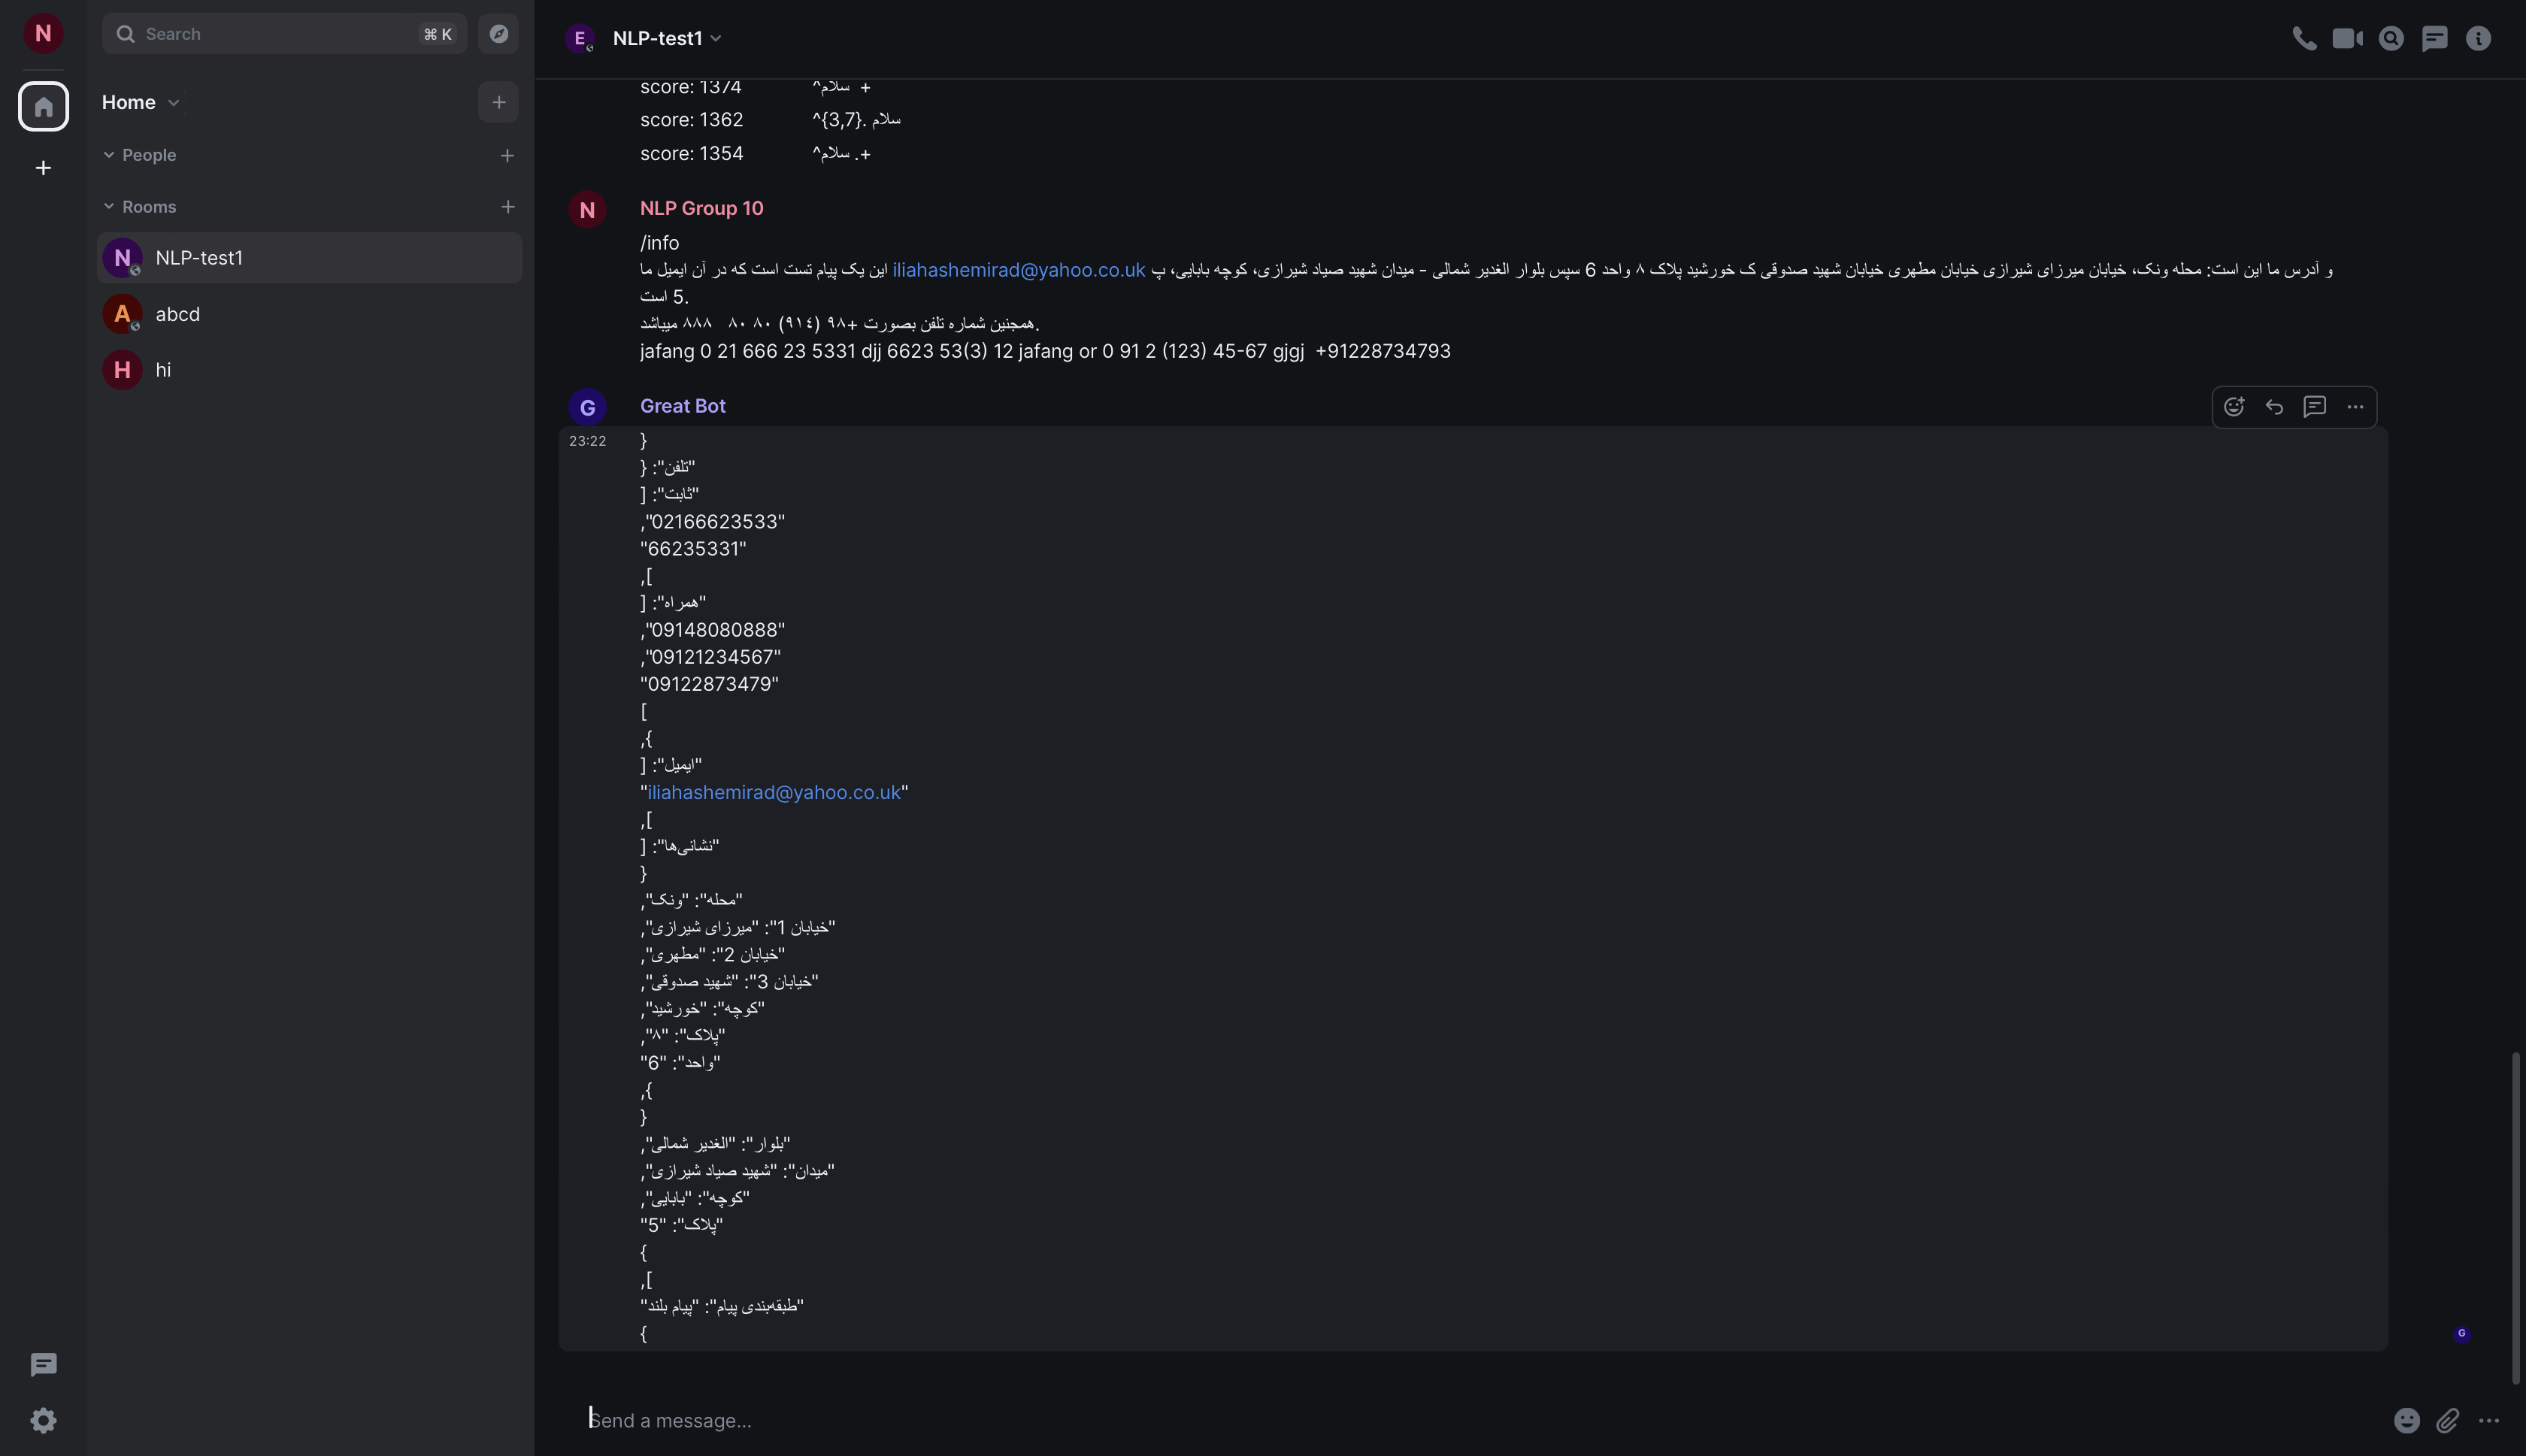
\includegraphics[scale = 0.3]{1.png}
\end{center}

\section{User Defined Regexes}
\begin{solution}
We used the SQLite3 database alongside the SQLalchemy package to store and use user-defined regexes in this part. This part's code is in the \verb*|database| directory.

At first, we define the database entity schema using the following code:
\end{solution}

\begin{lstlisting}[language=Python]
class MessagePattern(Base):
__tablename__ = 'message_patterns'
	id = Column(Integer, primary_key=True)
	name = Column(String, unique=True)
	regex = Column(String)
\end{lstlisting}

\begin{solution}
After that, we have two important functions, \verb*|add_regex| and \verb*|check_message_patterns|. The first one gets a name and regex as input, then adds that regex associated with that title to the database. It will also not allow duplicate titles and check uniqueness constraints. The latter runs a for loop on all patterns in the database and checks whether they match parts of the function input or not.\\

Here is some samples of testing this part:
\end{solution}

\begin{center}
  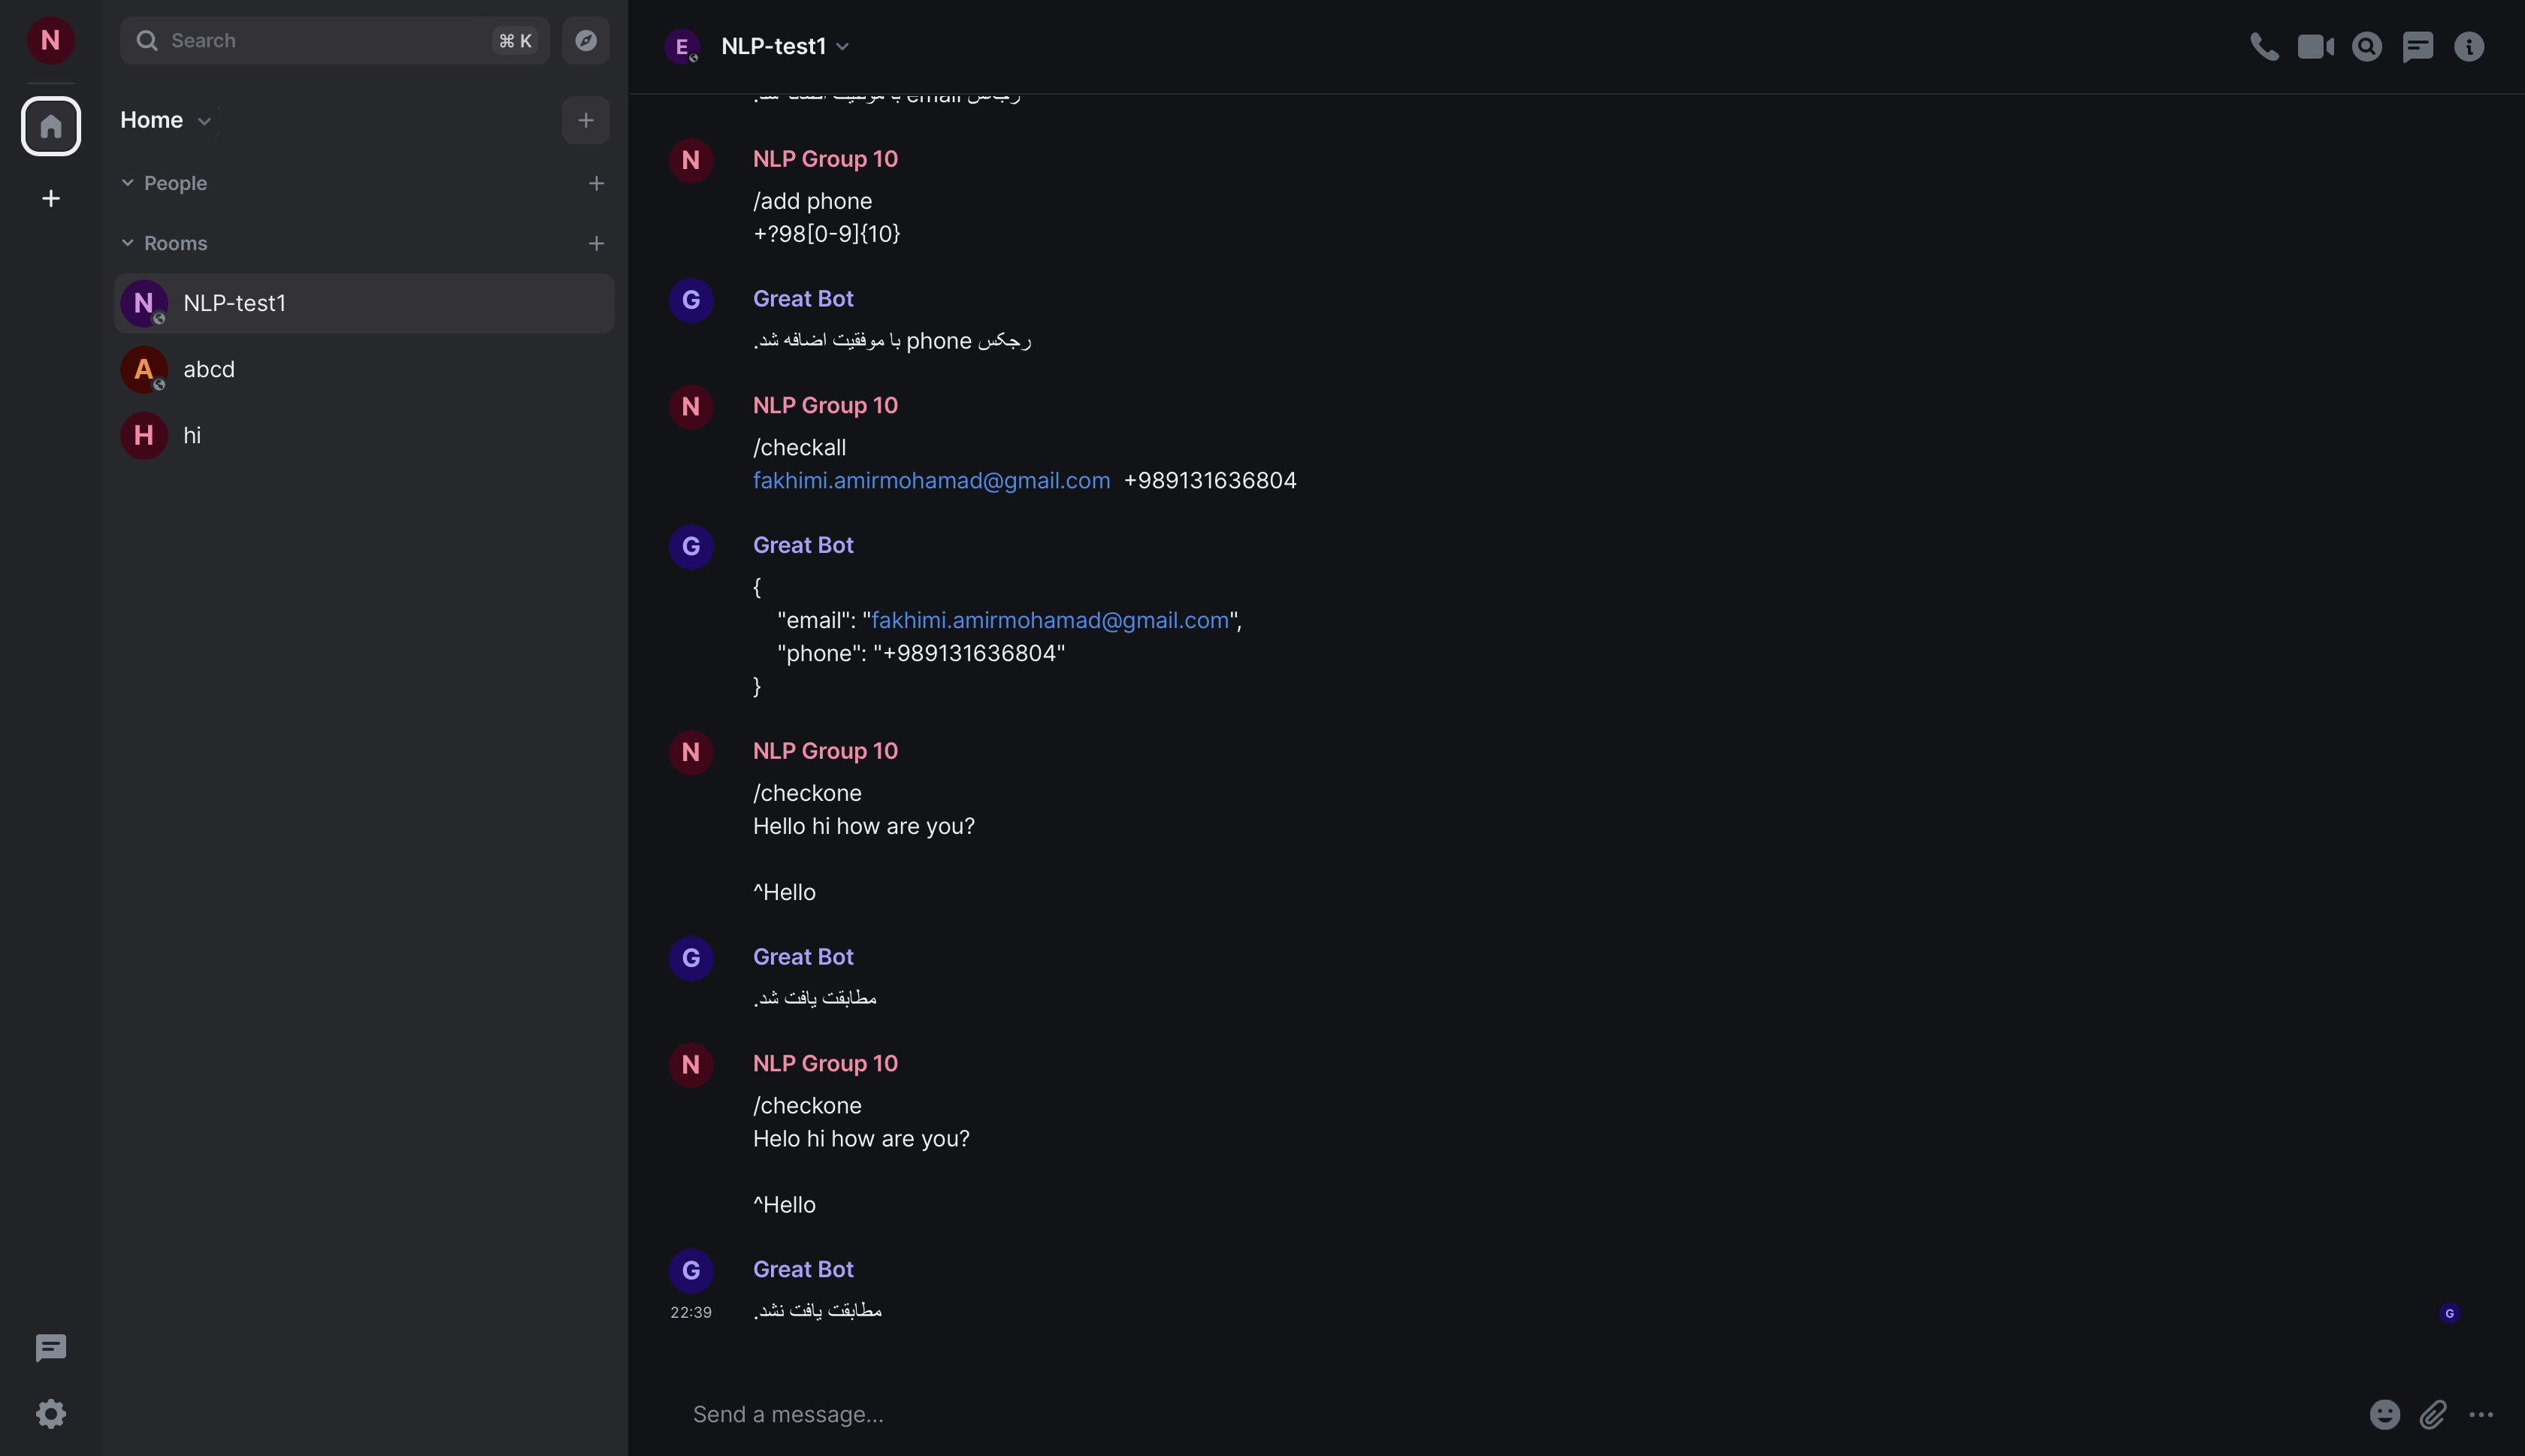
\includegraphics[scale = 0.3]{2.png}
\end{center}

\begin{center}
  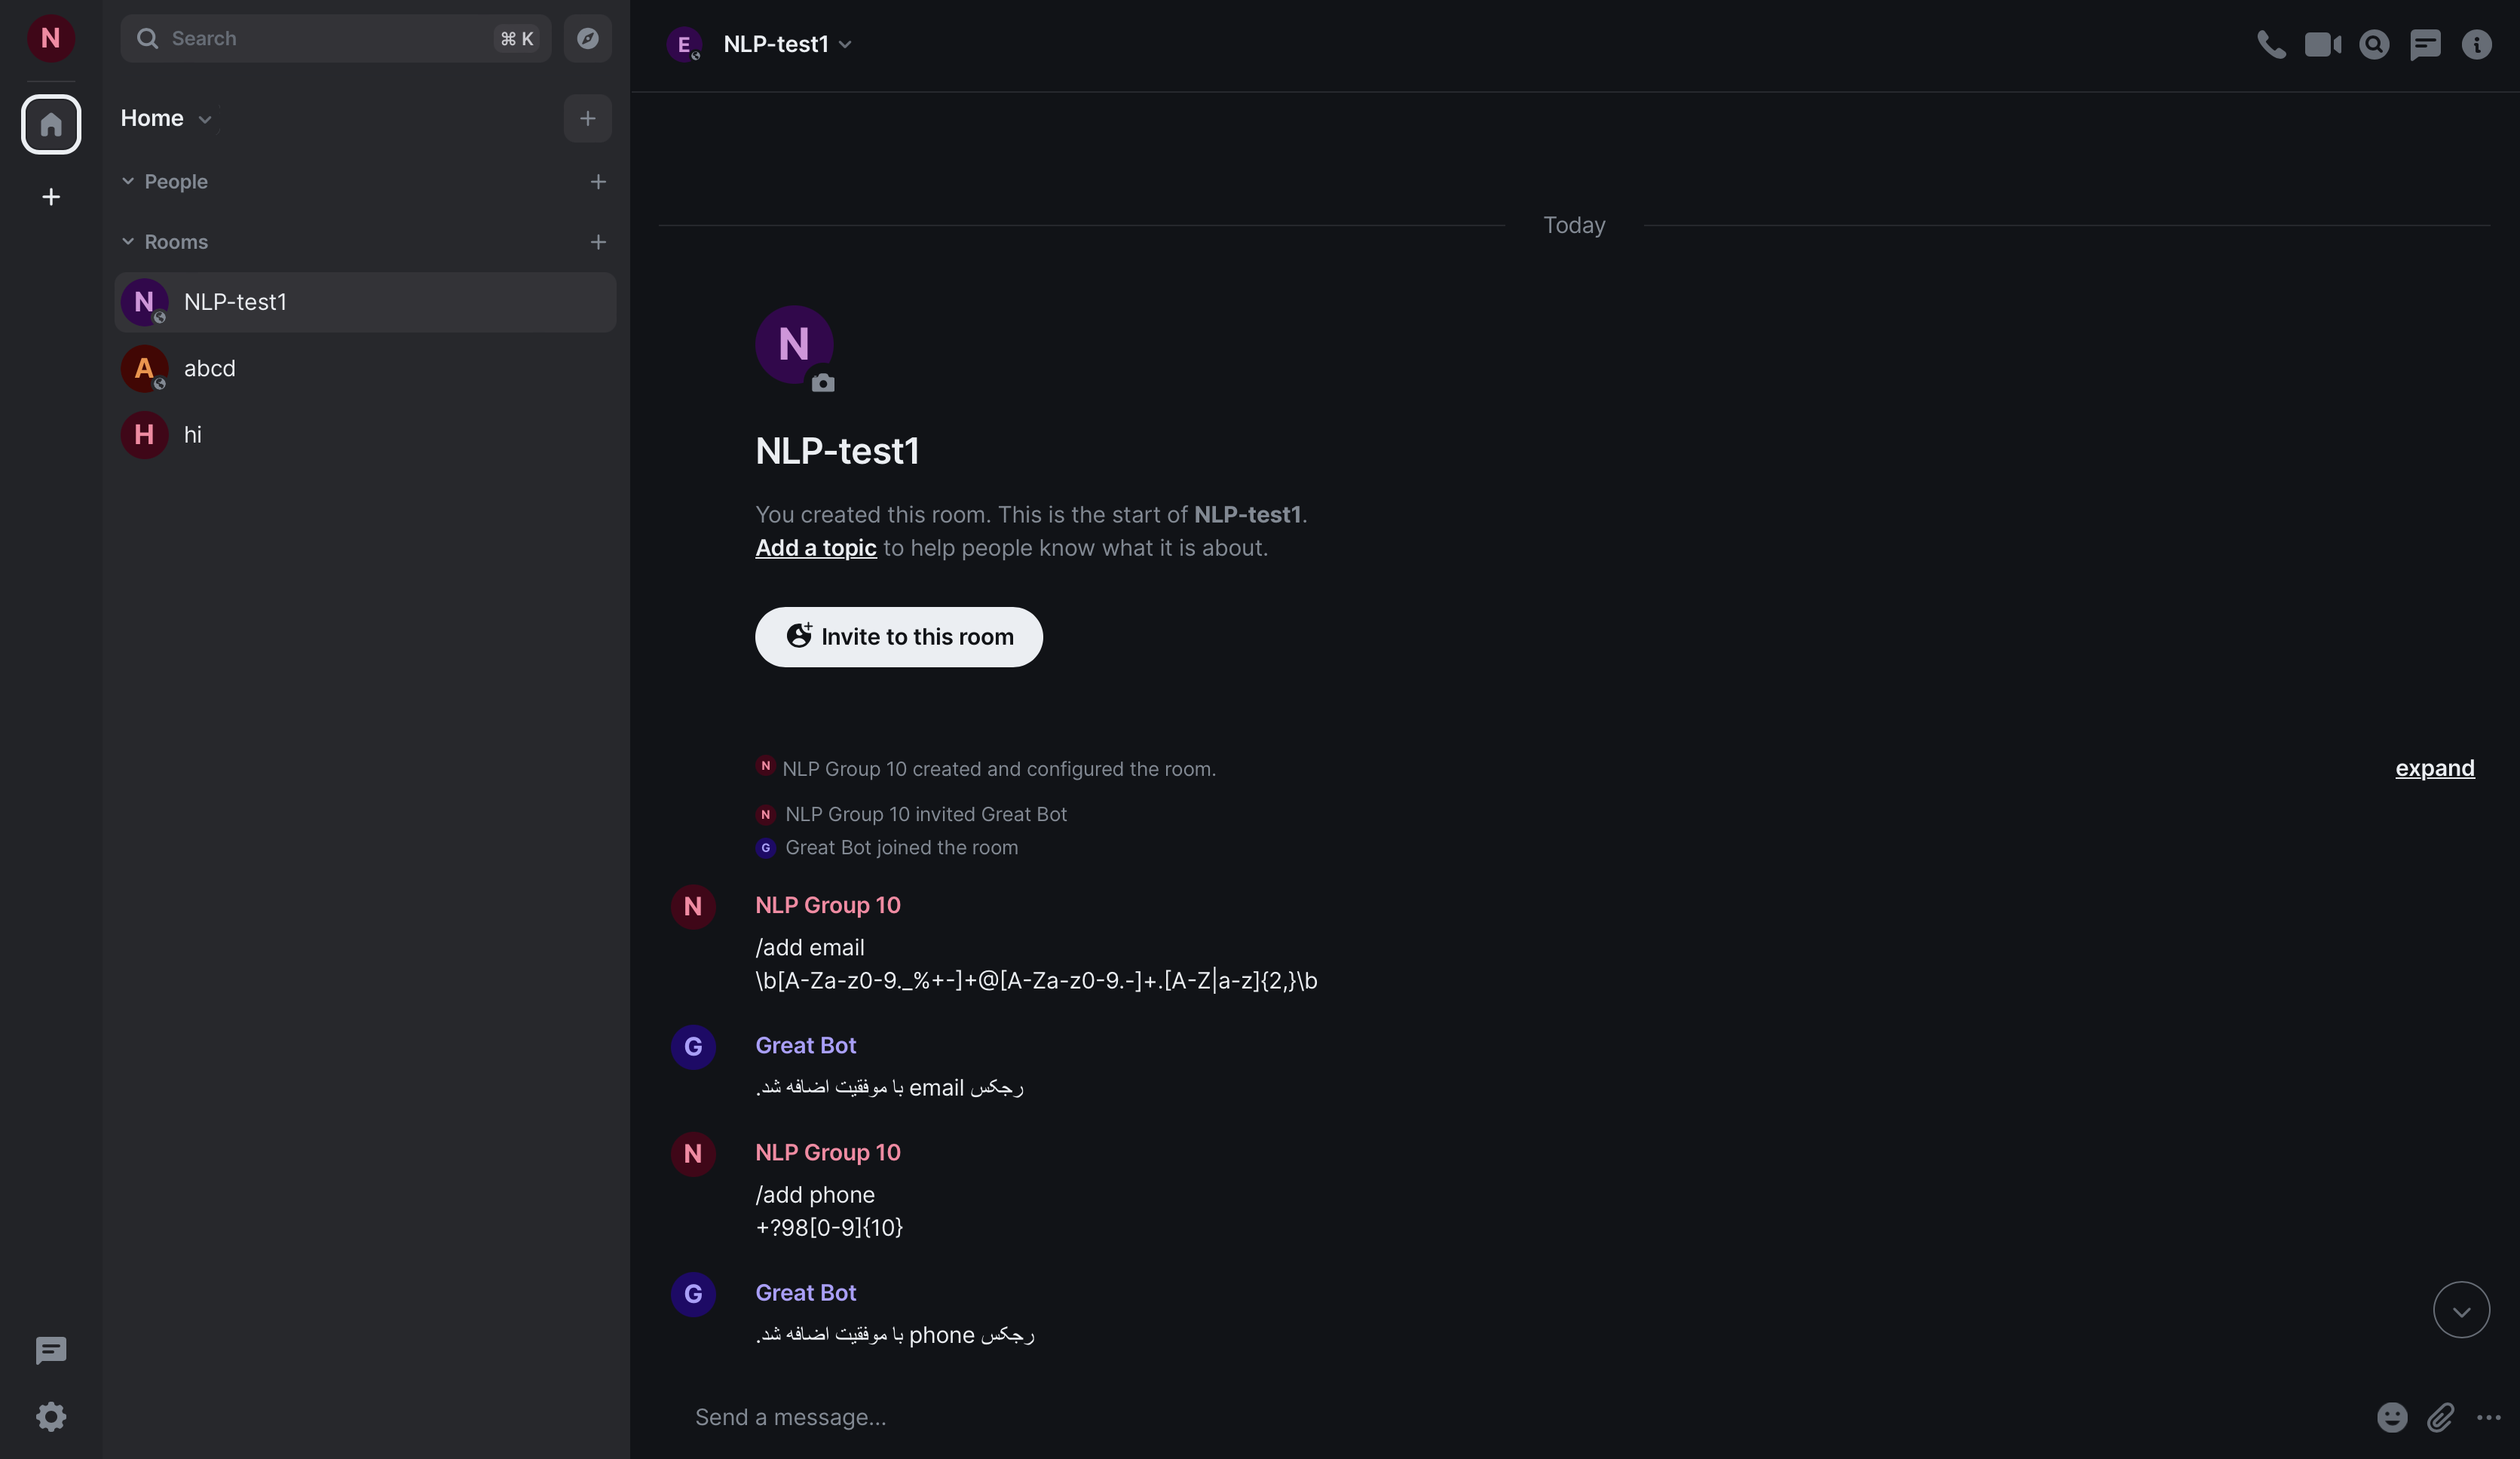
\includegraphics[scale = 0.3]{3.png}
\end{center}

\section{Genetic Algorithm}

\begin{solution}
For the regex extractor part of this project, we used genetic algorithms. Our main source for this part is from the paper we found in this GitHub repository: \url{https://github.com/maojui/Regex-Generator}.

The first part of the algorithm uses a preprocessor to extract all common sub-strings. Note that it does not just find the longest common sub-strings but uses a dynamic programming approach to find all common substrings. It then splits the string bases on these substrings. As this split could be done in different ways, it uses the way with the similarities between splits of each string.

After this preprocessing part, we define our genes based on widely used regex patterns. for example \verb*|\d| is corresponded to \verb*|0x0| genotype and \verb*|[A-Za-z]| is corresponded to \verb*|0x3|.  We modified the original code to add Persian language support.

With this definition, we encode our string into a phenotype by using our rules for genes. After that, we do some preprocessing sections to make the length of all phenotypes the same so they can be used in genetic algorithms. After that, we use typical genetic algorithms like substitution, crossover, and mutation to find the best match.

Our fitness function considers different parameters. The first and most important one is matching. The regex should match all the strings perfectly. If it does not match with one of the strings, it will get a score of minus infinity. Another factor is length, as we want to get short regexes. We will assign different penalties for using each gene. Broad-matching genes like "dot" are punished more harshly than specific genes.

With this in mind, we run different iterations of the genetic algorithm to get a reasonable result for our regex that matches all our strings.

The code is included in \verb*|regex_generator| directory and consists of multiple files. The important ones include:

\begin{enumerate}
\item \verb*|decoder.py|: This file is used to decode strings into phenotypes.

\item \verb*|evaluate.py|: This file includes functions that calculate fitness scores based on given regex/

\item \verb*|generator.py|: This file is the runner part of the algorithm that initiates the initial population and then runs the genetic algorithm.

\item \verb*|genetic.py|: This file include the main functions for genetic algorithm. Functions like mutation and crossover all reside in this file.

\item \verb*|parser.py|: This file includes the preprocessor part of our system that finds common substrings and does the string splitting based on these common substrings.

\end{enumerate}

Here is some samples of testing in this part:
\end{solution}

\begin{center}
  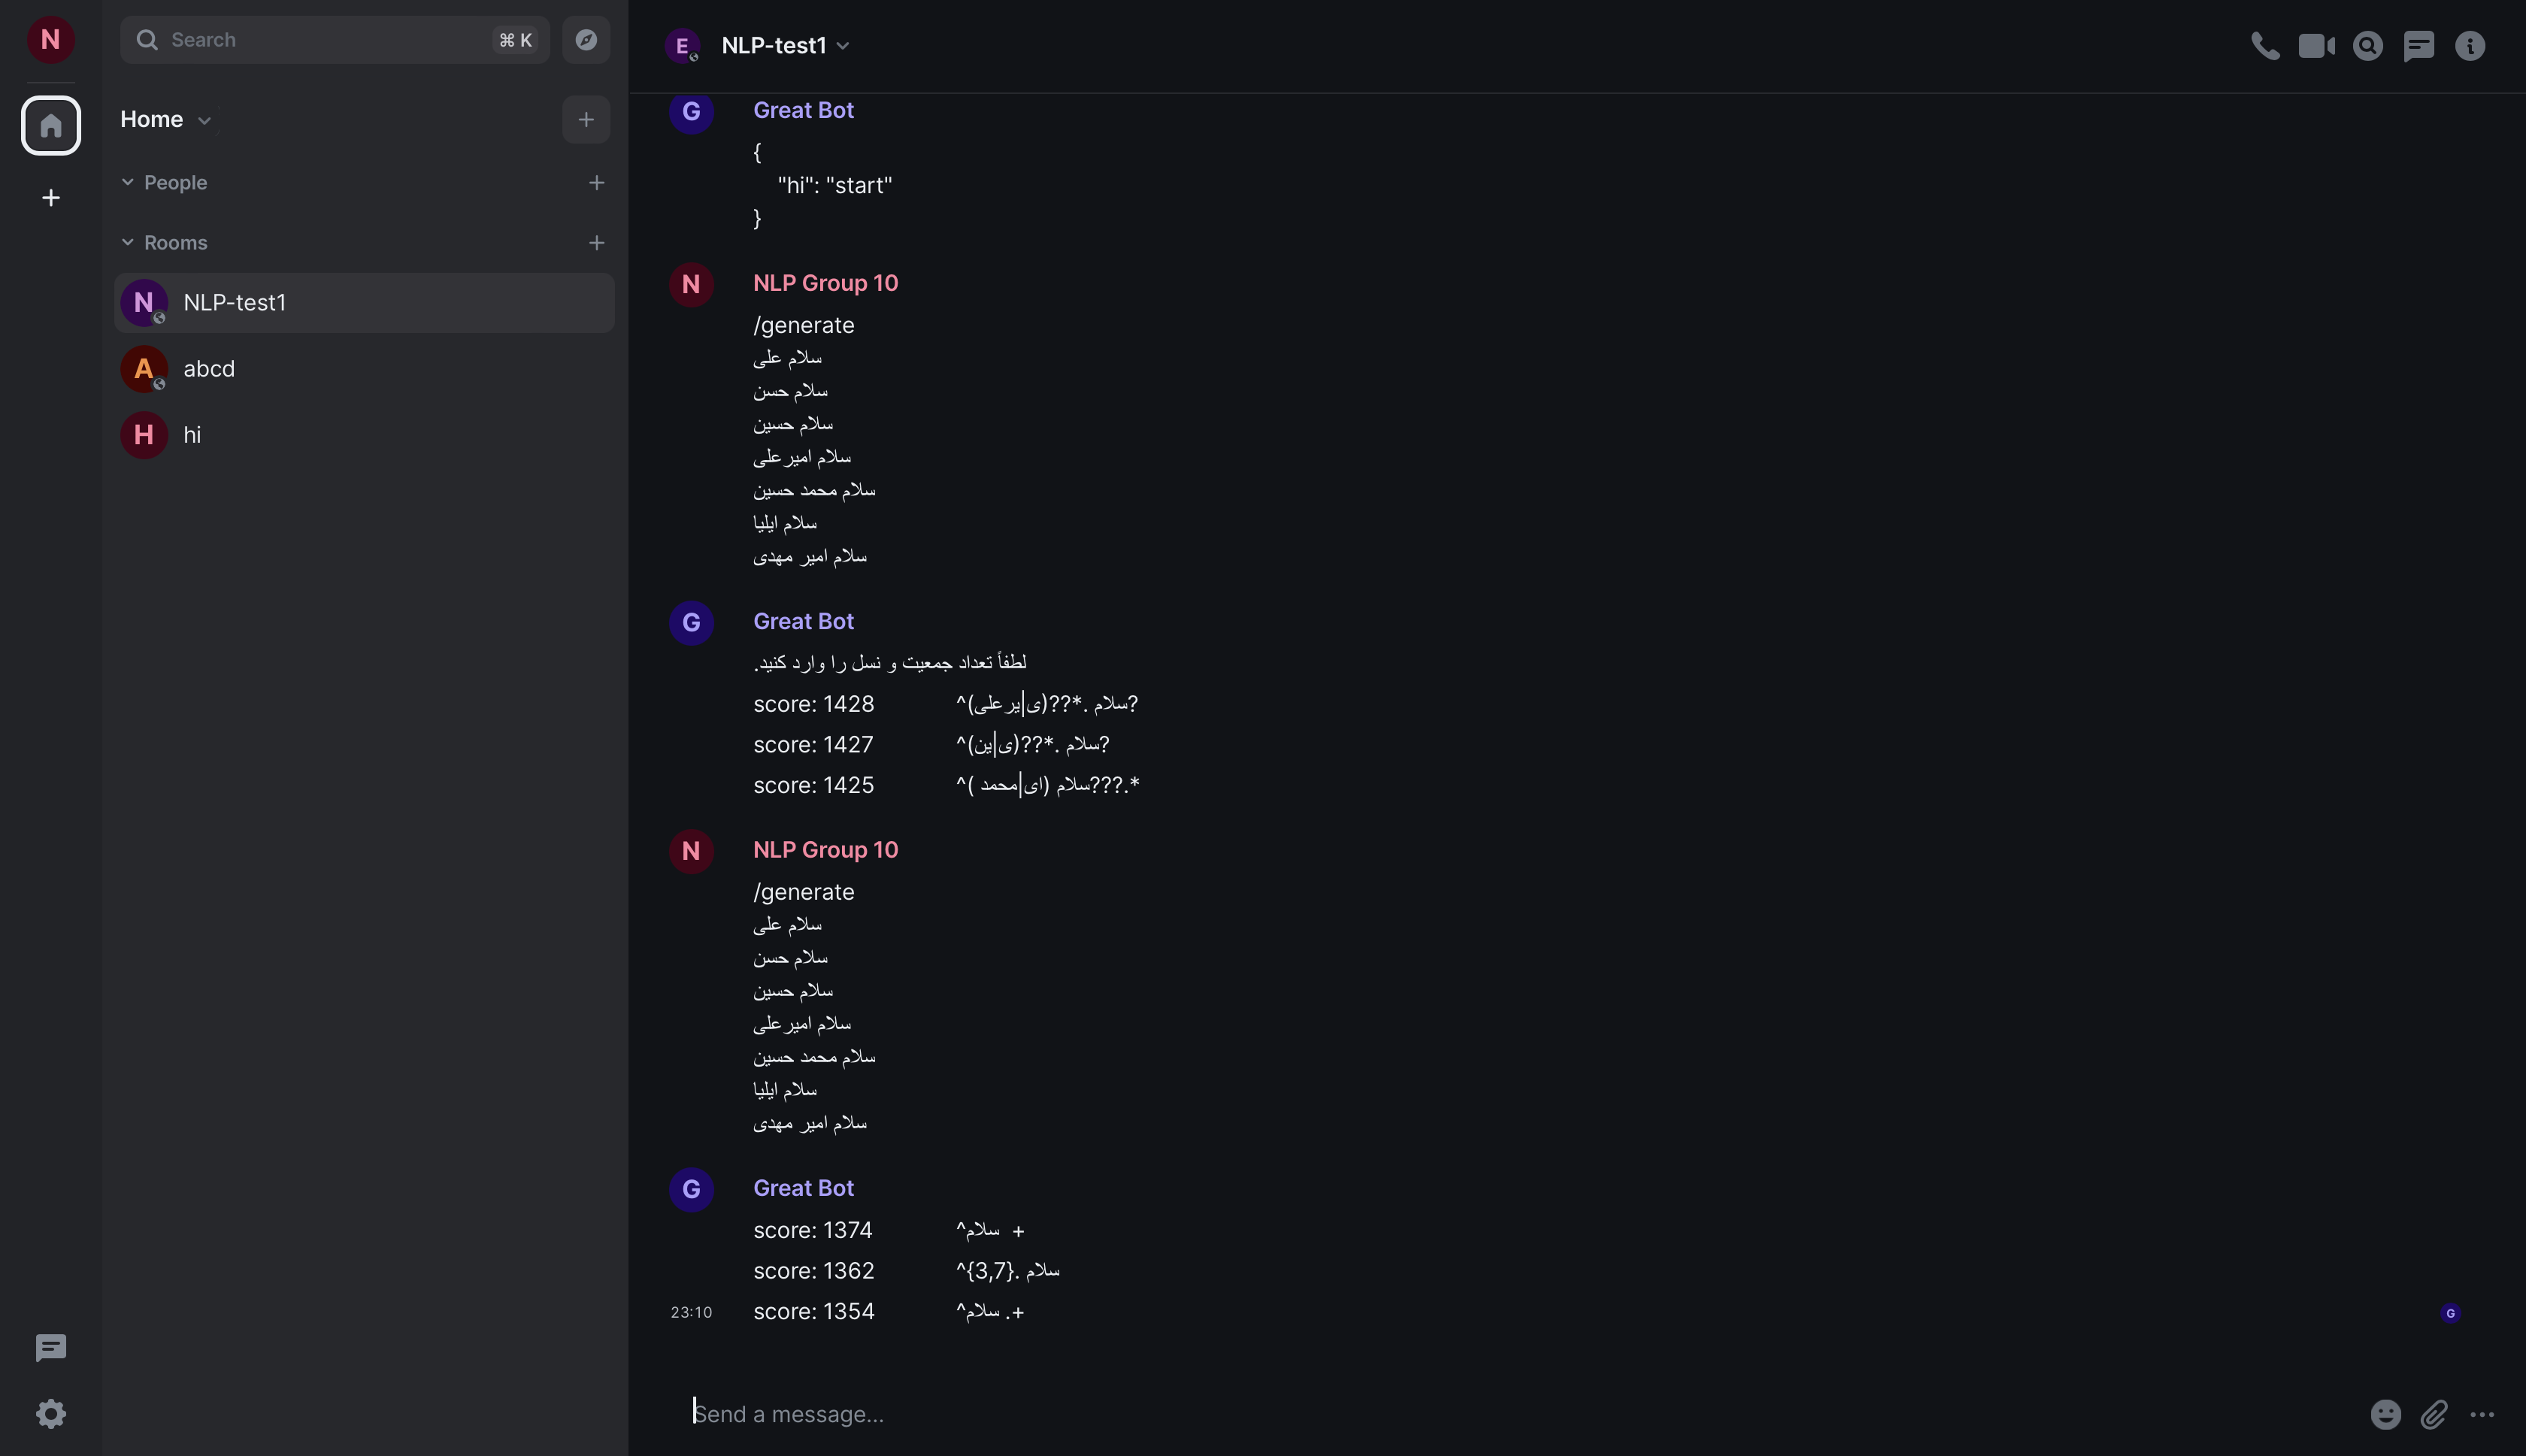
\includegraphics[scale = 0.3]{4.png}
\end{center}

%%%%%%%%%%%%%%%%%%%%%%%%%%%%%%%%%%%%%%%%%%%%%%%%%%%%%%%%%%%%
    % Add these commands below if it's not a problem for you
    \thispagestyle{fancyplain}
    \fancyhead{}
    \renewcommand{\headrulewidth}{0pt}
    %\rfoot{Template by L. R. Ximenes (Jimeens)}
%%%%%%%%%%%%%%%%%%%%%%%%%%%%%%%%%%%%%%%%%%%%%%%%%%%%%%%%%%%%
\end{document}












